\DiaryEntry{Convex Optimization, 2}{2015-12-07}{Optimization}

\subsection{Convex Optimization}

The generic (convex) optimization problem has the following form:


\begin{align*}
p^\star & = \min f(x) \\
f_i(x) & \leq 0 \, (i=1 \ldots m) \\
h_i(x) & = 0 \, (i=1 \ldots p) \\
\end{align*}


Points $x$ fulfilling these conditions are called feasible points; the set of all feasible points is the feasible set.

\subsection{Lagrangian Function}

We define the Lagrangian function as

\[
L(x,\lambda,\nu) = f(x) + \sum_i \lambda_i f_i(x) + \sum_i \nu_i h_i(x)
\]

The dual function of the optimization problem is

\[
g(\lambda, \nu) = \inf_x L(x,\lambda,\nu)
\]

Being a point-wise infinum of affine functions, the dual function is \textbf{always} concave, even if the original problem is not convex. The dual function yields a lower bound on $p^\star$; for $\lambda \geq 0 $ and any feasible point $\tilde x$ (therefore $f_i(\tilde x) < 0$ and $h_i(\tilde x)=0$) we have

\[
\sum_i \lambda_i f_i(\tilde x) + \sum_i \nu_i h_i(\tilde x) \leq 0
\]

Therefore

\[
g(\lambda, \nu) = \inf_x L(x,\lambda,\nu) \leq L(\tilde x, \lambda, \nu) \leq f(\tilde x)
\]

\subsubsection{Lagrange Dual Problem}

For $\lambda \geq 0$, the Lagrange dual gives a lower bound on the optimal value $p^\star$. This bound depends on $\lambda$ and $\nu$ and we can therefore ask for the optimal lower bound:


\begin{align*}
d^\star = \max & \, g(\lambda, \nu) \\
\text{s.t.} \lambda & \geq 0
\end{align*}


This is the Lagrange dual problem associated with the original optimization problem. The solution, the values $(\lambda^\star, \nu^\star)$, are the dual optimal or optimal Lagrange multipliers. We have $d^\star \leq p\star $; i.e.~the solution of the dual problem is less or equal the solution of the original optimization problem. The difference between these two, $p^\star - d^\star $, is called the duality gap. In case of weak duality, the duality gap is strictly larger than zero; in case of strong duality, we have $d^\star = p^\star $.

\subsection{Optimality Conditions (KKT Conditions)}

If $f_i$ are convex and $h_i$ are affine, then any points $\tilde x, \tilde \lambda, \tilde \nu$ satisfying


\begin{align}
\label{kkt1} f_i(\tilde x) & \leq 0 \\
\label{kkt2} g_i(\tilde x) & = 0 \\
\label{kkt3} \tilde \lambda_i & \geq 0 \\
\label{kkt4} \tilde \lambda_i f_i(\tilde x) & = 0 \\
\label{kkt5} \nabla f(\tilde x) + \sum_i \tilde \lambda_i \nabla f_i(\tilde x) + \sum_i \tilde \nu_i \nabla h_i(\tilde x) & = 0
\end{align}


are primal / dual optimal (with zero duality gap). Equations
$\eqref{kkt1}$ and $\eqref{kkt2}$ ensure that $\tilde x$ is feasible. $\eqref{kkt3}$ ensures that the Lagrangian is convex (in x); and $\eqref{kkt5}$ ensures that $\tilde x$ minimizes the Lagrangian over $x$.

\subsubsection{Example 1}

Consider the problem


\begin{align*}
\min f(x) &= x^2 \\
\text{s.t.} \, x-2 & \leq 0
\end{align*}


The Lagrangian becomes $L(x,\lambda) = x^2 + \lambda (x-2)$

The following figure shows the objective function (in red) and the
Lagrangian for increasing values of $\lambda$ (in blue). In the feasible region ( i.e.~for $x\leq 2$), the Lagrangian underestimates the objective function.

\begin{figure}[H]
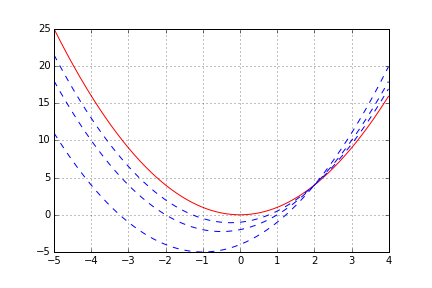
\includegraphics[scale=0.7]{images/convex_opt_03.png}
\end{figure}

The dual function is

\[
g(\lambda) = \inf_x L(x, \lambda) = \inf_x \big\{ x^2 + \lambda (x-2) \big\}
\]

Setting the derivative of $L$ with respect to $x$ to zero yields, $x=-\lambda/2$. Therefore, we have

\[
g(\lambda) = \left(-\frac{\lambda}{2}\right)^2 + \lambda \left( -\frac{\lambda}{2} - 2 \right) = - \frac{\lambda^2}{4} - 2\lambda
\]

The following plot shows the dual function $g(\lambda)$. Solving the dual problem $\eqref{dual}$; i.e.~maximizing $g(\lambda)$ with the constraint $\lambda > 0$ we see that the solution is $\lambda^\star = 0$ (yielding $d^\star = g(\lambda^\star)=0$).

\begin{figure}[H]
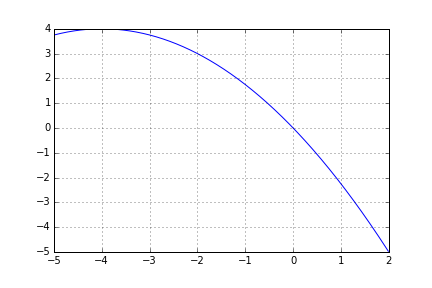
\includegraphics[scale=0.7]{images/convex_opt_03a.png}
\end{figure}

Using the KKT condition $\eqref{kkt5}$,

\[
\frac{dL}{dx} = 2x + \lambda = 0 \rightarrow x = - \frac{\lambda}{2}
\]

and the KKT condition $\eqref{kkt4}$ yields $\lambda(x-2) = 0$. From this last condition, we see two possible solutions: (A) $\lambda = 0 $ and (B) $x=2$. Starting with (A), it follows that $x=0$; for option (B) we have $\lambda=-4$. From $\eqref{kkt3}$ this is not allowed, therefore the (only) solution to the problem is $x=0$ and $\lambda=0$. This is also in line with the dual problem solved above; there we had that $\lambda^\star = 0$ and $d^\star = g(\lambda^\star)=0$).

The solution lies inside the feasible set; therefore the corresponding $\lambda$ equals zero.

If we consider


\begin{align*}
\min f(x) &= x^2 \\
\text{s.t.} \, x+2 & \leq 0
\end{align*}


instead, we get $L(x,\lambda) = x^2 + \lambda (x+2)$ and $\frac{dL}{dx} = 2x + \lambda = 0$.

The KKT condition $\eqref{kkt4}$ yields $\lambda(x+2) = 0$. Solution (A) becomes $\lambda = 0$ and $x=0$; solution (B) becomes $\lambda = 4$ and $x=-2$. Solution (A) violates feasibility $\eqref{kkt1}$, therefore the (only) solution is $\lambda = 4$ and $x=-2$. In this case, the solution lies at the border of the feasible region, therefore the corresponding Lagrangian $\lambda$ is unequal zero.

\begin{figure}[H]
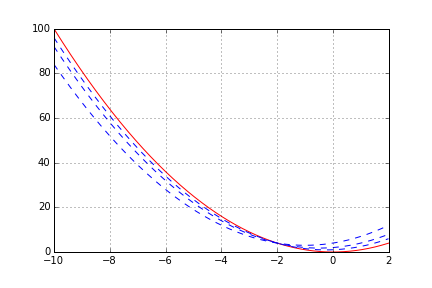
\includegraphics[scale=0.7]{images/convex_opt_04.png}
\end{figure}

The dual function is

\[
g(\lambda) = \inf_x L(x, \lambda) = \inf_x \big\{ x^2 + \lambda (x+2) \big\} = -\frac{\lambda^2}{4} + 2\lambda
\]

which is shown below.

\begin{figure}[H]
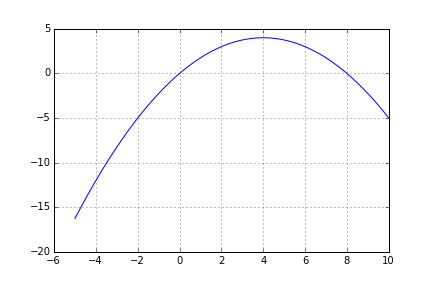
\includegraphics[scale=0.7]{images/convex_opt_04a.png}
\end{figure}

Maximizing (for positive $\lambda$) we have $\lambda^\star=4$ and $d^\star = g(\lambda^\star) = 4$ - again this is in line with the solution of the original problem above.

\subsubsection{Interpretation}

The Lagrangian can be interpreted as follows: Actually we want to
minimize the function

\[
f(x) + \sum_i \mathcal{I}_-(f_i(x)) + \sum_i \mathcal{I}_0(h_i(x))
\]

where the indicator functions are defined as

\[
\mathcal{I}_-(u)=
\begin{cases}
0, \quad u \leq 0 \\
\infty , \quad u > 0
\end{cases}
\]

and

\[
\mathcal{I}_0(u)=
\begin{cases}
0, \quad u = 0 \\
\infty , \quad u \neq 0
\end{cases}
\]

These indicator functions describes the ``displeasure'' with the
equality / inequality constraints: if they are violated, our displeasure is infinite; otherwise we are not unsatisfied. The two $\mathcal{I}_-, \mathcal{I}_0$ are brick-wall functions; even a small violation yields radical displeasure. If we instead use linear displeasure functions, we arrive at the Lagrangian. The more inequality and equality constraints are violated, the larger the two sum terms $ \sum\_i \lambda\_i f\_i(x) + \sum\_i \nu\_i h\_i(x) $ become.

The solution $\tilde x$ of the optimization problem is either (i) inside the feasible region or (ii) located at the border of the feasible region.

In the first case, the derivative of the objective function alone
vanishes because $\tilde x$ is an optimum; i.e. $\nabla f(\tilde x) = 0$. However, the derivative of the Lagrangian $L(x,\lambda,\nu) = f(x) + \sum_i \lambda_i f_i(x) + \sum_i \nu_i h_i(x)$ will \textbf{not} vanish, because the inequality constraints are less than zero in the feasible region: $f_i(\tilde x)\leq 0$. For the
KKT condition $\eqref{kkt5}$ to hold, the Lagrangian multipliers $\lambda$ must be zero.

In the second case, the derivative of the objective function alone will \textbf{not} vanish; for example see the second example above. In this case, the Lagrangian multipliers $\lambda$ will be unequal zero, so that the derivative of the Lagrangian is zero.

If considering problems with order higher than one, these considerations apply for each dimension - see the next example.

\subsubsection{Example 2}

This time consider a two-dimensional function


\begin{align*}
\min f(x,y) &= x^2 + y^2 \\
\text{s.t.} \, 1-x & \leq 0 \\
-1-y & \leq 0
\end{align*}


The Lagrangian is $L = x^2 + y^2 + \lambda_1(1-x) + \lambda_2(-1-y)$. Taking derivatives, we obtain


\begin{align*}
\frac{\partial L}{\partial x} & = 2x - \lambda_1 \\
\frac{\partial L}{\partial y} & = 2y - \lambda_2
\end{align*}


Considering $\lambda_1(1-x)=0$, we have $\lambda_1=0, x=0$ which is not a solution as it is not a feasible point. The other solution, $\lambda_1=2, x=1$ is a valid solution. From $\lambda_2(-1-y)=0$ we find that $\lambda_2=0, y=0$ is a feasible point, whereas $\lambda_2=-2, y=-1$ is not.

This example is a case where the solution for the x-axis is constrained by an inequality constraint, therefore the corresponding
$\lambda_1 \neq 0$. The solution alone the y-axis is not constrained, therefore the corresponding $\lambda_2 = 0$.

The contour plot is given below with the black point ($x=1, y=0$) being the solution.

\begin{figure}[H]
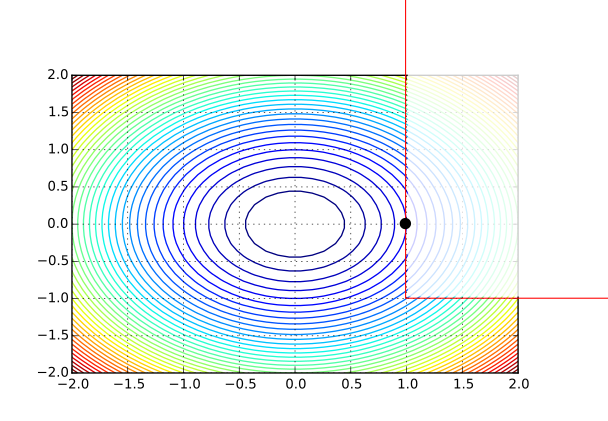
\includegraphics{images/convex_opt_05.png}
\end{figure}
